\section{Introducción}

Consideremos la secci\'on horizontal de un horno de acero cil\'indrico, como en la Figura 1. El sector A es la pared del horno, y el sector B es el horno propiamente dicho, en el cual se funde el acero a temperaturas elevadas. Tanto el borde externo como el borde interno de la pared forman c\'irculos. Suponemos que la temperatura del acero dentro del horno (o sea, dentro de B) es constante e igual a 1500$^{o}$C.

\medskip

Tenemos sensores ubicados en la parte externa del horno para medir la temperatura de la pared externa del mismo, que habitualmente se encuentra entre 50$^{o}$C y 200$^{o}$C. El problema que debemos resolver consiste en estimar la isoterma de 500$^{o}$C dentro de la pared del horno, para estimar la resistencia de la misma. Si esta isoterma est\'a demasiado cerca de la pared externa del horno, existe peligro de que la estructura externa de la pared colapse.

\begin{figure}[ht]
\begin{center}
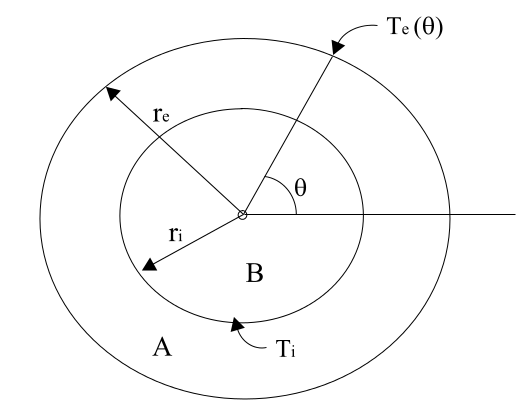
\includegraphics[width=0.4\columnwidth]{catedra/Horno.png}
\caption{Secci\'on circular del horno}
\end{center}
\end{figure}

Sea $r_e \in \mathbb{R}$ el radio exterior de la pared y sea $r_i \in \mathbb{R}$ el radio interior de la pared. Llamemos $T(r,\theta)$ a la temperatura en el punto dado por las coordenadas polares $(r,\theta)$, siendo $r$ el radio y $\theta$ el angulo polar de dicho punto. En el estado estacionario, esta temperatura satisface la ecuación del calor dada por el laplaciano:

\begin{equation}\label{calor}
\frac{\partial^2T(r,\theta)}{\partial r^2}+\frac{1}{r}\frac{\partial T(r,\theta)}{\partial r}+\frac{1}{r^2}\frac{\partial^2T(r,\theta)}{\partial \theta^2} = 0 
\end{equation}

Para resolver esta ecuación de forma numérica, discretizamos la superficie de la pared y luego aproximamos las derivadas parciales:

\begin{figure}[ht]
\begin{center}
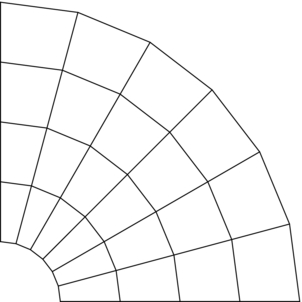
\includegraphics[width=0.2\columnwidth]{catedra/disc.png}
\caption{Discretizacion de la pared del horno.}
\end{center}
\end{figure}

\begin{equation}
\frac{\partial^2T(r,\theta)}{\partial r^2}(r_j,\theta_k) \cong \frac{t_{j-1,k}-2t_{jk}+t_{j+1,k}}{(\Delta r)^2}
\end{equation}

\begin{equation}
\frac{\partial T(r,\theta)}{\partial r}(r_j,\theta_k) \cong \frac{t_{j,k}-t_{j-1,k}}{\Delta r}
\end{equation}

\begin{equation}
\frac{\partial^2T(r,\theta)}{\partial \theta^2}(r_j,\theta_k) \cong \frac{t_{j,k-1}-2t_{jk}+t_{j,k+1}}{(\Delta \theta)^2}
\end{equation}

Reemplazando la aproximación numérica en el laplaciano y el radio por su respectiva discretizacion obtenemos:
\begin{equation}\label{calor}
\frac{t_{j-1,k}-2t_{jk}+t_{j+1,k}}{(\Delta r)^2}
+ \frac{1}{r_j}
\frac{t_{j,k}-t_{j-1,k}}{\Delta r}
+
\frac{1}{r_j^2}
\frac{t_{j,k-1}-2t_{jk}+t_{j,k+1}}{(\Delta \theta)^2} = 0
\end{equation}

Donde $r_j = r_i + j \times \Delta\theta$.

Por lo tanto, aproximamos de forma discreta la ecuación diferencial dada por el laplaciano.


Si llamamos $T_i \in \mathbb{R}$ a la temperatura en el interior del horno (sector B) y $T_e : [0,2\pi] \rightarrow \mathbb{R}$ a la función de temperatura en el borde exterior del horno (de modo tal que el punto $(r_e,\theta)$ tiene temperatura $T_e(\theta)$), entonces tenemos que

\begin{equation}
T(r,\theta) = T_i \;\;\;\;\;para\;todo\;punto\;(r,\theta)\;con\;r\leq r_i
\end{equation}
\begin{equation}
T(r_e,\theta) = T_e(\theta) \;\;\;\;\;\;para\;todo\;punto\;(r_e,\theta)
\end{equation}

\subsection{Discretizacion}

Para resolver este problema computacionalmente, discretizamos el dominio del problema (el sector A) en coordenadas polares. Consideramos una partici\'on $0 = \theta_0 < \theta_1 < ... < \theta_n = 2\pi$ en $n$ \'angulos discretos con $\theta_k-\theta_{k-1} = \Delta\theta$ para $k = 1,...,n$, y una partici\'on $r_i = r_0 < r_1 < ... < r_m = r_e$ en $m+1$ radios discretos con $r_j - r_{j-1} = \Delta r$ para $j = 1,...,m$.

De esta manera, terminamos con un sistema de $(m-1)*(n+1)$ ecuaciones lineales, que puede ser experesado como $Ax = b$. Para cada temperatura $t_{j,k}$, tendremos un laplaciano. Esto no sucede con los valores de las temperaturas en las puntas, donde ya a priori sabemos el valor final $t_i$ y $t_s(\theta)$. Estas temperaturas en las puntas formaran parte del vector de valores independientes b al armar el sistema. La discretizacion muchas veces depende de los valores anteriores y posteriores, por lo que hay que tener cuidado de no caer en uno de estos casos borde al formular el sistema.

\subsection{Sistema Lineal}
Para formular el sistema lineal, en primer lugar debemos despejar cada una de las variables $t_{j,k}$ de la aproximación discreta del laplaciano:

\begin{equation}\label{calor}
\frac{t_{j-1,k}-2t_{j,k}+t_{j+1,k}}{(\Delta r)^2}
+ \frac{1}{r_j}
\frac{t_{j,k}-t_{j-1,k}}{\Delta r}
+
\frac{1}{r_j^2}
\frac{t_{j,k-1}-2t_{j,k}+t_{j,k+1}}{(\Delta \theta)^2} = 0
\end{equation}

Reescribiendo:

\begin{equation}
\alpha_{j,k} \times t_{j,k} + \alpha_{j-1,k} \times t_{j-1,k} + \alpha_{j+1,k} \times t_{j+1,k} + \alpha_{j,k+1} \times t_{j,k+1} + \alpha_{j,k-1} \times t_{j,k-1} = 0
\end{equation}

Donde:

\begin{equation}
\alpha_{j,k} = \frac{-2}{(\Delta r)^2} + \frac{1}{r_j \times \Delta r} + \frac{-2}{r_j^2 \times (\Delta \theta)^2}
\end{equation}

\begin{equation}
\alpha_{j,k+1} = \frac{1}{r_j^2 \times (\Delta \theta)^2}
\end{equation}

\begin{equation}
\alpha_{j,k-1} = \frac{1}{r_j^2 \times (\Delta \theta)^2}
\end{equation}

\begin{equation}
\alpha_{j+1,k} = \frac{1}{(\Delta r)^2}
\end{equation}

\begin{equation}
\alpha_{j-1,k} = \frac{1}{(\Delta r)^2} - \frac{1}{r_j \times \Delta r}
\end{equation}

\subsection{Isoterma}
Una vez que resolvamos el sistema lineal, debemos buscar la isoterma. Dada que es una aproximación discreta, no es muy probable que encontremos valores de temperatura justo iguales a la curva de nivel. Por lo tanto debemos tener cierta tolerancia de error, o hasta interpolar de alguna manera curvas de nivel adyacentes. Es decir, debemos hacer una búsqueda inteligente sobre el vector $b$. De hecho, dado que el calor se propaga de forma uniforme, podríamos hasta interpolar un circulo con las temperaturas adyacentes. La única forma de que la isoterma tenga una forma elíptica es que la temperatura exterior no sea uniforme. En este caso, simplemente hay que interpolar una elipse.